\documentclass[11pt]{article}
\usepackage{amsmath, amssymb, amsthm}
\usepackage[retainorgcmds]{IEEEtrantools}

\usepackage{tikz}
\usetikzlibrary{intersections, decorations.pathreplacing}

\usepackage{fancyhdr}

%Listings stuff
\usepackage{listings}
\usepackage{lstautogobble}
\usepackage{color}

\definecolor{gray}{rgb}{0.5,0.5,0.5}
\lstset{
basicstyle={\small\ttfamily},
tabsize=3,
numbers=left,
numbersep=5pt,
numberstyle=\tiny\color{gray},
stepnumber=2,
breaklines=true,
boxpos=t
}

%Format stuff
\pagestyle{fancy}
\headheight 35pt

%Header info
\chead{\Large \textbf{Stable Matching}}
\lhead{}
\rhead{}

\begin{document}
\section{Problem}
	Given two sets $M$ of ``men'' and $W$ of ``women'', where for each $m \in M$ and $w \in W$, there exists a complete sequence of preferences of members of the other set, find a mutually agreeable perfect matching.
	
	\subparagraph{Stability} Mutually agreeable in this context is defined to be a matching with no \textbf{instability}. An unstable matching is defined as one with at least 1 pair of matches $(m, w)$ and $(m', w')$ such that $m$ prefers $w'$ to $w$ and $m'$ prefers $w$ to $w'$. In this instance, all parties involved have an incentive to work outside the system and ``elope''.
	
	Consider the following diagram:
	
	\begin{center}
	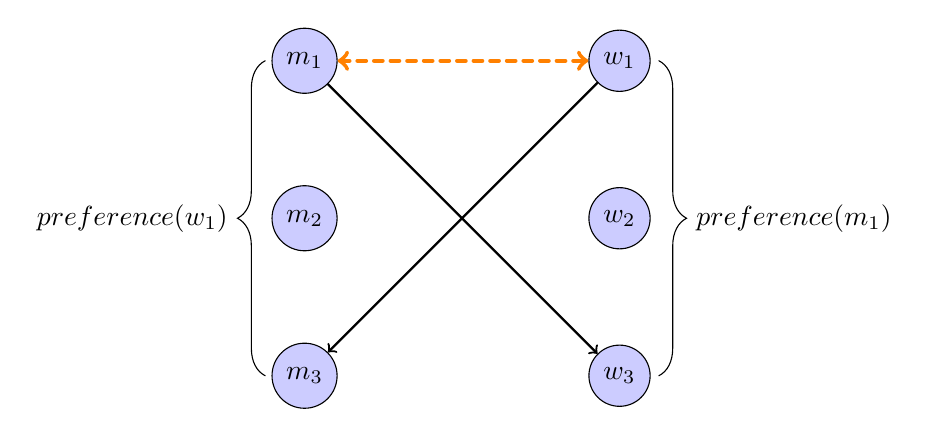
\begin{tikzpicture}
		[scale=2,line cap=round,
		%Styles
		axes/.style=,
		important line/.style={very thick},
		information text/.style={rounded corners,fill=red!10,inner sep=1ex},
		dot/.style={circle,inner sep=1pt,fill,label={#1},name=#1},
		main node/.style={circle,fill=blue!20,draw}			
		]
		
		%Colors
		\colorlet{anglecolor}{green!50!black}	%angle arcs/lines
		
		%The graphic
		
		\node[main node] (M1) at (0, 0) {$m_1$};
		\node[main node] (M2) at (0, -1) {$m_2$};
		\node[main node] (M3) at (0, -2) {$m_3$};
		
		\node[main node] (W1) at (2, 0) {$w_1$};
		\node[main node] (W2) at (2, -1) {$w_2$};
		\node[main node] (W3) at (2, -2) {$w_3$};
		
		\path[->, thick]
			(M1)	edge	(W3)
			(W1)	edge	(M3);
		
		\path[<->, dashed, ultra thick, orange]
			(M1)	edge	(W1);
			
		\draw[decorate,decoration={brace,amplitude=10pt,mirror}] (-.25, 0) -- node[left=10pt] {$preference(w_1)$} (-.25, -2);
		
		\draw[decorate, decoration={brace,amplitude=10pt}] (2.25, 0) -- node[right=10pt] {$preference(m_1)$} (2.25, -2);
	\end{tikzpicture}
	\end{center}
	In this case, because $m_1$ and $w_1$ mutually prefer each other to their currently matched partners, the matching is instable.
	
\section{Algorithm}
	The Gale-Shapley algorithm (1962) computes a perfect stable matching for the problem in polynomial (technically linear) time.
	
	\begin{lstlisting}[autogobble=true,mathescape]
		Initialize all m $\in$ M and w $\in$ W to free
		while $\exists$ free m who still has a woman w to propose to:
			if w is free:
				engage (m, w)
			else:
				let m' be current partner of w
				if w prefers m to m':
					free m'
					engage (m, w)
	\end{lstlisting}
	
	 Essentially, the men iteratively take turns proposing to women by order of preference, and the women can reject, accept, and switch partners based on their preferences. Note that while the solution is stable, it may not necessarily produce an optimal matching from the women's point of view, because while the men have the entire set of women to choose from, the women only get to choose between a limited subset of the men at any given time.
	 
\section{Runtime}
	Once a man proposes to a woman, he will never propose to her again. She may reject his proposal right now or in the future, but he will only move further down his preference list. Therefore, each man will propose at most $n$ times (all the way through the preference list). Because there are $n$ men in the input, the algorithm runs in $O(n^2)$ time.
	
	However, because each man and woman has a complete preference list, we can say that the input size is actually $2n^2$. Therefore, the Gale-Shapley algorithm runs in linear time.
	
\section{Proof}
	The proof comes in two parts: first, prove that the G-S algorithm produces a perfect matching (no unmatched people), and next, prove that the matching will always be stable.
	
	\subparagraph{Proof of Perfect Matching} On termination, if some man $m$ ends up without a woman, he must have proposed to and been rejected by every woman in his preferece list. There will also exist some $w \in W$ that is unengaged. Note that once a woman is engaged, she stays engaged for the whole algorithm (although her man can change), so this means that $w$ must have been unproposed to. 
	
	However, because preference lists must be complete, $w$ must have been in $m$'s preference list, which leads to a contradiction because $m$ must have proposed to every woman in his list for an imperfect matching to exist. By contradiction, the G-S algorithm therefore produces a perfect matching every time.
	
	\subparagraph{Proof of Stability} Suppose, in the output, there exists some instability as below:
	
	\begin{center}
	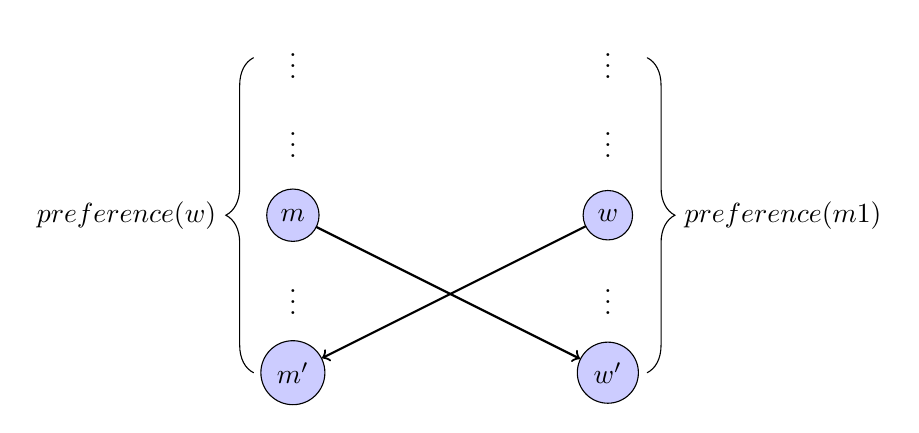
\begin{tikzpicture}
		[scale=2,line cap=round,
		%Styles
		axes/.style=,
		important line/.style={very thick},
		information text/.style={rounded corners,fill=red!10,inner sep=1ex},
		dot/.style={circle,inner sep=1pt,fill,label={#1},name=#1},
		main node/.style={circle,fill=blue!20,draw}			
		]
		
		%Colors
		\colorlet{anglecolor}{green!50!black}	%angle arcs/lines
		
		%The graphic
		\node[draw=none] (ellipsis1) at (0, 0) {$\vdots$};
		\node[draw=none] (ellipsis2) at (0, -.5) {$\vdots$};
		\node[main node] (M) at (0, -1) {$m$};
		\node[draw=none] (ellipsis3) at (0, -1.5) {$\vdots$};
		\node[main node] (Mp) at (0, -2) {$m'$};
		
		\node[draw=none] (ellipsis1) at (2, 0) {$\vdots$};
		\node[draw=none] (ellipsis2) at (2, -.5) {$\vdots$};
		\node[main node] (W) at (2, -1) {$w$};
		\node[draw=none] (ellipsis3) at (2, -1.5) {$\vdots$};
		\node[main node] (Wp) at (2, -2) {$w'$};
		
		\path[thick,->]
			(M)	edge	(Wp)
			(W)	edge	(Mp);
			
		\draw[decorate,decoration={brace,amplitude=10pt,mirror}] (-.25, 0) -- node[left=10pt] {$preference(w)$} (-.25, -2);
		
		\draw[decorate, decoration={brace,amplitude=10pt}] (2.25, 0) -- node[right=10pt] {$preference(m1)$} (2.25, -2);
	\end{tikzpicture}
	\end{center}
	
	Before proposing to $w'$, $m$ must have proposed to $w$ in this situation, because a man's partner only gets worse as the algorithm goes on. This means that $w$ must have rejected $m$ initially because she was paired with a more preferential mate $m''$, or broke off her engagement to $m$ in favor of $m''$.
	
	However, $m' < m < m''$, and since $w$ would have been engaged to $m''$ at some point, she could never be proposed to $m'$ because she either would have rejected him immediately or switched partners. By contradiction therefore, the G-S algorithm produces a stable matching.

%	\begin{center}
%	\begin{tikzpicture}
%		[scale=3,line cap=round,
%		%Styles
%		axes/.style=,
%		important line/.style={very thick},
%		information text/.style={rounded corners,fill=red!10,inner sep=1ex},
%		dot/.style={circle,inner sep=1pt,fill,label={#1},name=#1}			
%		]
%		
%		%Colors
%		\colorlet{anglecolor}{green!50!black}	%angle arcs/lines
%		
%		%The graphic
%	\end{tikzpicture}
%	\end{center}

%	\begin{figure}[htb]
%		\centering
%		\includegraphics[width=0.8\textwidth]{filename.eps}
%		\caption{Caption.}
%		\label{fig:figure}
%	\end{figure}

%		\def\enotesize{\normalsize}
%		\theendnotes
\end{document}